\documentclass[border=4pt,12pt]{standalone}
% House style for redrawn exam diagrams (diagram-v4: 0.4pt lines, filled -latex arrows, fine dashes; stipple and hatching drawn as real dots/lines (no PDF/SVG patterns, so they render in every browser and at any scale); transparent background). Every figure \input's this.
\usepackage{amsmath,amssymb}
\usepackage{txfonts}
\usepackage{pdfrender,xcolor}
% \halo{text}: label on shading. The shading stops just around each letter's outline (a thin knock-out that follows the
% glyphs, like the papers' typesetting), never a box. Owner: "I don't want a box around the text".
\newcommand{\halo}[1]{\leavevmode\rlap{\pdfrender{TextRenderingMode=2,LineWidth=2.2pt,LineJoinStyle=1,StrokeColor=white,FillColor=white}#1}#1}
\usepackage{tikz,pgfplots}
\pgfplotsset{compat=1.18}
\usetikzlibrary{arrows.meta,calc,angles,quotes,patterns,patterns.meta,intersections,positioning,decorations.markings,shapes.geometric}
% Stipple and hatching are drawn as actual dots / lines clipped to the region (path picture), NOT as pattern fills:
% SVG <pattern> fills vanish or blur when browsers scale the image, so the owner could not see the shading.
% Each dot is a 0.72pt square (keeps SVGs small; reads as a dot at print size). Dots sit on one global staggered grid, so neighbouring regions line up.
\makeatletter
\newdimen\ex@x \newdimen\ex@y \newdimen\ex@xa \newdimen\ex@ya \newdimen\ex@xb \newdimen\ex@yb \newcount\ex@row
\def\exam@stipplecolor{black!75}\def\exam@dotr{0.42pt}\def\exam@dotgap{2.5}
\def\ex@rowdots{\ifdim\ex@x<\ex@xb \pgfpathrectangle{\pgfqpoint{\dimexpr\ex@x-0.36pt\relax}{\dimexpr\ex@y-0.36pt\relax}}{\pgfqpoint{0.72pt}{0.72pt}}\advance\ex@x by \exam@dotgap pt\relax\expandafter\ex@rowdots\fi}
\def\exam@stipple{%
  \pgftransformreset% dots are sized in real points even inside scaled pictures
  \pgfpointanchor{path picture bounding box}{south west}\ex@xa=\pgf@x \ex@ya=\pgf@y
  \pgfpointanchor{path picture bounding box}{north east}\ex@xb=\pgf@x \ex@yb=\pgf@y
  \pgfsetfillcolor{\exam@stipplecolor}\pgfmathsetmacro\ex@h{\exam@dotgap/2}%
  \pgfmathtruncatemacro\ex@r{floor(\ex@ya/\ex@h)-1}\ex@row=\ex@r\relax
  \ex@y=\ex@r\dimexpr\ex@h pt\relax
  \loop\ifdim\ex@y<\ex@yb
    \pgfmathtruncatemacro\ex@c{floor(\ex@xa/\exam@dotgap)-1}\ex@x=\ex@c\dimexpr\exam@dotgap pt\relax
    \ifodd\ex@row \advance\ex@x by \ex@h pt\fi
    \ex@rowdots
    \advance\ex@y by \ex@h pt \advance\ex@row by 1
    \ifnum\numexpr\ex@row-(\ex@row/4)*4\relax=0 \pgfusepath{fill}\fi% flush every 4 rows: bounded TeX memory, few clip copies in the SVG
  \repeat\pgfusepath{fill}}
\newdimen\ex@d
\def\exam@hatch#1{% #1 = 1 for /, -1 for \ ; lines 45 degrees, 3pt apart
  \pgftransformreset
  \pgfpointanchor{path picture bounding box}{south west}\ex@xa=\pgf@x \ex@ya=\pgf@y
  \pgfpointanchor{path picture bounding box}{north east}\ex@xb=\pgf@x \ex@yb=\pgf@y
  \ex@d=\dimexpr\ex@yb-\ex@ya\relax \ex@x=\dimexpr\ex@xa-\ex@d\relax
  \loop\ifdim\ex@x<\ex@xb
    \ifnum#1>0 \pgfpathmoveto{\pgfqpoint{\ex@x}{\ex@ya}}\pgfpathlineto{\pgfqpoint{\dimexpr\ex@x+\ex@d\relax}{\ex@yb}}%
    \else \pgfpathmoveto{\pgfqpoint{\ex@x}{\ex@yb}}\pgfpathlineto{\pgfqpoint{\dimexpr\ex@x+\ex@d\relax}{\ex@ya}}\fi
    \advance\ex@x by 4.24pt
  \repeat
  \pgfsetlinewidth{0.4pt}\pgfsetstrokecolor{black}\pgfusepath{stroke}}
\def\examstipple{\exam@stipple}\def\examhatch{\exam@hatch}\def\examsetstipplecolor#1{\def\exam@stipplecolor{#1}}\def\examsetdotgap#1{\def\exam@dotgap{#1}}
\makeatother
% (legacy pattern kept for old files)
% staggered stipple like the NESA papers' dotted shading
\pgfdeclarepatternformonly{exam stipple}{\pgfpointorigin}{\pgfqpoint{2.2pt}{2.2pt}}{\pgfqpoint{2.2pt}{2.2pt}}{%
  \pgfpathcircle{\pgfqpoint{0.55pt}{0.55pt}}{0.42pt}\pgfpathcircle{\pgfqpoint{1.65pt}{1.65pt}}{0.42pt}\pgfusepath{fill}}
\tikzset{
  every picture/.style={line width=0.6pt, >={Latex[length=2mm,width=1.3mm]}},
  curve/.style={line width=0.6pt},
  open arrow/.style={-{Latex[length=2mm,width=1.3mm]}},  % owner: filled -latex heads everywhere, no open chevrons
  aux/.style={dash pattern=on 2pt off 1.5pt, line width=0.6pt},
  shade/.code={\def\exA{#1}\def\exB{none}\ifx\exA\exB\else\pgfkeysalso{fill=black!18}\fi},
  shade/.default=on,
  shade dots/.style={fill=none, path picture={\examstipple}},
  stipple color/.code={\examsetstipplecolor{#1}},
  stipple gap/.code={\examsetdotgap{#1}},
  shade dense dots/.style={fill=none, stipple gap=1.6, path picture={\examstipple}},
  shade hatch/.style={fill=none, path picture={\examhatch{1}}},
  shade hatch reverse/.style={fill=none, path picture={\examhatch{-1}}},
  shade solid/.style={fill=black},
  pt/.style={circle, fill, inner sep=1.1pt},
  open pt/.style={circle, draw, fill=white, inner sep=1.1pt},
}
\pgfplotsset{
  exam axes/.style={axis lines=middle, axis line style={->}, xlabel={$x$}, ylabel={$y$},
    xlabel style={anchor=west}, ylabel style={anchor=south}, tick label style={font=\small},
    every axis plot/.append style={line width=0.6pt, black}, samples=200, clip=false,
    enlargelimits=false, axis on top},
}

\begin{document}
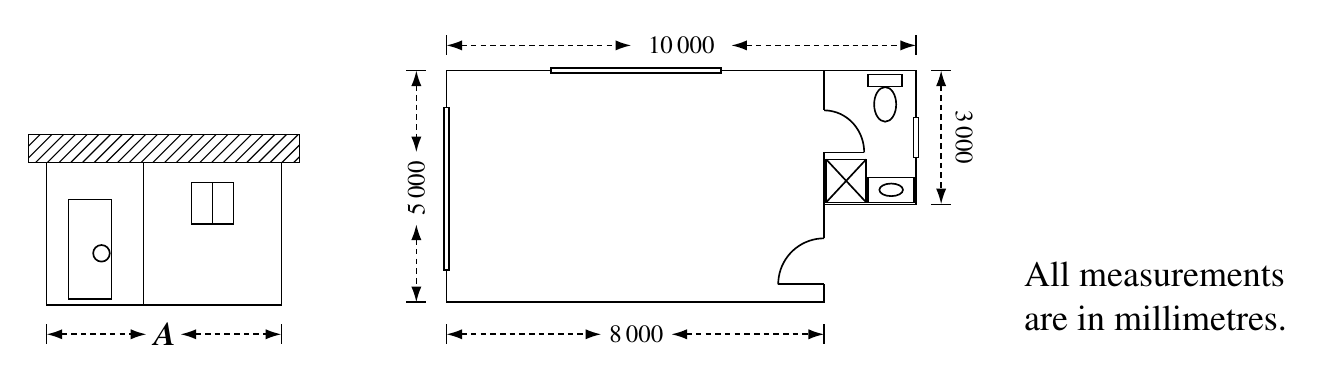
\begin{tikzpicture}[x=0.0127cm,y=-0.0127cm]
% ---- elevation
\path[shade hatch] (22,122) rectangle (293,150);
\draw (22,122) rectangle (293,150);
\draw (40,150) -- (40,293) -- (275,293) -- (275,150);
\draw (137,150) -- (137,293);
\draw (62,187) rectangle (105,287);
\draw (95,241) circle (3pt);
\draw (185,170) rectangle (227,212); \draw (206,170) -- (206,212);
\draw (40,312) -- (40,332); \draw (275,312) -- (275,332);
\draw[aux,<->] (40,322) -- (140,322);
\draw[aux,<->] (174,322) -- (275,322);
\node[font=\large] at (157,322) {$\boldsymbol{A}$};
% ---- floor plan walls
\draw (545,58) -- (440,58) -- (440,95);
\draw (440,258) -- (440,290) -- (818,290) -- (818,272);
\draw (818,226) -- (818,192) -- (910,192) -- (910,145);
\draw (910,105) -- (910,58) -- (715,58);
\draw (818,58) -- (818,98);
\draw (818,140) -- (818,192);
% windows
\draw (545,55.5) rectangle (715,60.5);
\draw (437.5,95) rectangle (442.5,258);
\draw (907.5,105) rectangle (912.5,145);
% doors (leaf + swing arc centred on the hinge)
\draw (818,140) -- (858,140);
\draw plot[smooth,samples=20,domain=0:90] ({818+40*cos(\x)},{140-42*sin(\x)});
\draw (818,272) -- (772,272);
\draw plot[smooth,samples=20,domain=90:180] ({818+46*cos(\x)},{272-46*sin(\x)});
% bathroom fittings
\draw (820,147) rectangle (860,190); \draw (820,147) -- (860,190); \draw (860,147) -- (820,190);
\draw (862,165) rectangle (908,190); \draw (885,177.5) ellipse (0.15cm and 0.08cm);
\draw (862,62) rectangle (896,74); \draw (879,92) ellipse (0.14cm and 0.22cm);
% dimensions
\begin{scope}[font=\small]
\draw (440,23) -- (440,43); \draw (910,23) -- (910,43);
\draw[aux,<->] (440,33) -- (625,33); \draw[aux,<->] (725,33) -- (910,33);
\node at (675,33) {$10\,000$};
\draw (400,58) -- (420,58); \draw (400,290) -- (420,290);
\draw[aux,<->] (410,58) -- (410,140); \draw[aux,<->] (410,212) -- (410,290);
\node[rotate=90] at (410,176) {$5\,000$};
\draw (925,58) -- (945,58); \draw (925,192) -- (945,192);
\draw[aux,<->] (935,58) -- (935,192);
\node[rotate=-90] at (958,125) {$3\,000$};
\draw (440,312) -- (440,332); \draw (818,312) -- (818,332);
\draw[aux,<->] (440,322) -- (595,322); \draw[aux,<->] (665,322) -- (818,322);
\node at (630,322) {$8\,000$};
\end{scope}
\node[align=left,anchor=west,font=\fontsize{13}{16}\selectfont] at (1008,284) {All measurements\\are in millimetres.};
\end{tikzpicture}
\end{document}